\section {Grundlagen}
\subsection{ROS2}
\ac{ROS2} ist eine Sammlung von Bibliotheken und Werkzeugen für Robotik-Applikationen welche alle OpenSource sind.
Die erste \ac{ROS2} Release-Version erschien im Dezember 2017 unter dem Namen Ardent Apalon \citet{ros2docs}.\\
Es werden  mehrere \acp{RCL}  zur Verfügung gestellt, welche den Zugriff auf die \ac{ROS2}-API ermöglichen.
Die \acp{RCL} für die Sprachen C++ und Python (rclcpp und rclpy) werden dabei direkt vom \ac{ROS2}-Team verwaltet.
Von der Community wurden weitere \acp{RCL}, unter anderem für die Sprachen C\#, Swift und Rust, entwickelt.\\
Um die Entwicklung der \acp{RCL} zu vereinfachen und die Logik sprachen unabhängig zu machen werden Funktionalitäten als C Interfaces zugänglich gemacht, für welche in den \acp{RCL} Wrapper geschrieben werden.
\subsubsection{Node}
Nodes sind die grundlegenden Komponenten, aus welchen eine \ac{ROS2} Anwendung besteht.
Typischerweise besteht eine Anwendung aus mehreren Nodes.
Entsprechend dem Prinzip Separation of Concerns (Trennung der Zuständigkeiten) sollen Nodes so implementiert werden, dass sie jeweils nur eine spezifische Aufgabe haben.
\subsection{ROS2 Interfaces}
In diesem Abschnitt werden die verschiedenen Arten von Interfaces beschrieben, welche für die im folgenden Abschnitt~\ref{rosnodecomm} erklärten Methoden zur Kommunikation zwischen mehreren Nodes genutzt werden.\\
\ac{ROS2} Interfaces sind Definitionen, welche Daten mit welchen Typen gesendet werden.
Sie werden in der \ac{IDL} geschrieben, welche es ermöglicht automatisch Source Code in verschiedenen Sprachen für diese zu generieren.\\
- Erklären was für den build nötig ist?
\subsubsection{Message}
Eine Message ist der einfachste Typ der \ac{ROS2} Interfaces, welcher gleichzeitig auch ein Baustein für die folgenden Interfaces sein wird.\\
Message Definitionen haben die Dateiendung \verb|.msg| und werden per Konvention in einem Ordner \verb|msg/| gespeichert.
Jede \verb|.msg| Datei besteht aus den folgenden Teilen:
\begin{itemize}
\item Felder
\item Konstanten
\end{itemize}
Jedes Feld besteht aus einem Typ und einem durch ein Leerzeichen getrennten Namen: \verb|typ name|, z.B. \verb|bool isDone|.
Als Typ können dabei die integrierten Typen (s. Tabelle~\ref{tab:builtintypes}) oder der Name anderer Messages genutzt werden.
Zusätzlich kann jeder integrierte Typ als Array definiert werden (s. Tabelle~\ref{tab:arraytypes}).\\
Feldnamen müssen kleingeschrieben sein.
Es können alphanumerische Zeichen sowie der Unterstrich zur Trennung von Wörtern genutzt werden.
Das erste Zeichen muss ein Buchstabe sein und der Name darf nicht mit einem Unterstrich enden.
Zusätzlich darf es keine aufeinander folgenden Unterstriche geben.\\
Konstanten behalten das Format der Felder bei.
Der Name der Konstante wird komplett in Großbuchstaben geschrieben.
Zusätzlich bekommen Konstanten einen Wert zugewiesen, welcher nicht innerhalb des Programms geändert werden kann.
Die Zuweisung des Wertes erfolgt mit dem \verb|=| Zeichen: \verb|string EXAMPLE="test"|.
\begin{table}[ht]
    \centering
    \caption{Integrierte Datentypen für Interfaces und deren C++ Equivalent}
\begin{tabular}{|l|l|}
\hline
\textbf{Typ} & \textbf{C++}   \\ \hline
bool         & bool           \\ \hline
byte         & uint8\_t       \\ \hline
char         & char           \\ \hline
float32      & float          \\ \hline
float64      & double         \\ \hline
int8         & int8\_t        \\ \hline
uint8        & uint8\_t       \\ \hline
int16        & int16\_t       \\ \hline
uint16       & uint16\_t      \\ \hline
int32        & int32\_t       \\ \hline
uint32       & uint32\_t      \\ \hline
int64        & int64\_t       \\ \hline
uint64       & uint64\_t      \\ \hline
string       & std::string    \\ \hline
wstring      & std::u16string \\ \hline
\end{tabular}
    \label{tab:builtintypes}
\end{table}
\begin{table}[ht]
    \centering
    \caption{Array Typen und deren C++ Equivalent}
\begin{tabular}{|l|l|}
\hline
\textbf{Typ} & \textbf{C++}   \\ \hline
static array               & std::array<T, N>   \\ \hline
unbounded dynamic array    & std::vector        \\ \hline
bounded dynamic array      & custom\_class<T, N> \\ \hline
bounded string             & std::string        \\ \hline
\end{tabular}
    \label{tab:arraytypes}
\end{table}
\subsubsection{Service}
Service Definitionen beschreiben eine Anfrage und eine Antwort.
Die Definition hat die Dateiendung \verb|.srv| und wird im Ordner \verb|srv/| gespeichert.
Anfrage und Antwort werden innerhalb der Datei durch \verb|-| getrennt.
Für beide Teile gilt, dass sie gültig sind, wenn sie einer gültigen Message Definition entsprechen.
Ein Beispiel einer einfachen Servicedefinition ist in Listing~\ref{lst:serviceexample} zu sehen.\\
\begin{minipage}{\linewidth}%minipage to prevent page break
\begin{lstlisting}[caption={Beispiel einer Service Definition}, label={lst:serviceexample}]
int32 request_int
string request_string
---
float32 response_float
\end{lstlisting}
\end{minipage}
\subsubsection{Action}
Action Definitionen bestehen aus den 3 Teilen Anfrage, Ergebnis und Feedback, in dieser Reihenfolge.
Wie auch für Service Definitionen gilt, das die Teile durch \verb|-| getrennt sind und jeder einzelne Teil gültig ist, wenn er einer gültigen Message Definition entspricht.
\subsection{ROS2 Node Kommunikation}{\label{rosnodecomm}}
Damit verschiedene Nodes untereinander kommunizieren können, gibt es verschieden Mechanismen, welche sich primär darin unterscheiden, in welche Richtungen Nachrichten gesendet werden und ob es eine direkte Reaktion gibt.
Für alle Mechanismen gilt, das sie von einer Node unter einem bestimmten Namen sowie einem Typ zur Verfügung gestellt werden und von anderen Nodes durch eben diese genutzt werden können.
\subsubsection{Topic}
Topics entsprechen in etwa einem Newsletter System: eine Node veröffentlicht Daten, welche von allen anderen Nodes empfangen wird, die sich für diese registriert haben.
Das Format der Daten entspricht einer gewählten Message Definition.
\subsubsection{Service und Client}
Services werden für Prozesse genutzt, in denen eine Anfrage gesendet und eine Antwort erwartet wird.
Als Typ wird eine Servicedefinition genutzt.
\subsubsection{Action Server und Client}
Actions sind für länger andauernde Prozesse gedacht.
Eine Node erstellt einen Action Server über welchen eine Action zur Verfügung gestellt wird.
Andere Nodes können über einen Action Client eine Anfrage senden.
Der Server bearbeitet die Anfrage und sendet bei Beendigung eine Antwort mit einem Ergebnis an den Client.
Während der Dauer der Action kann der Server den Client optional mit Feedback Nachrichten über den aktuellen Status informieren.\\
Als Typ wird eine Action Definition genutzt. 
\subsection{OpenMANIPULATOR-X}
Der OpenMANIPULATOR-X ist ein von der Firma ROBOTIS{\footnote{http://en.robotis.com}} nach den Prinzipien ``OpenSoftware`` und ``OpenHardware`` hergestellter Greifarm.
OpenSoftware steht hierbei dafür, dass es ein OpenSource Projekt ist und auf dem OpenSource Projekt \ac{ROS2} basiert.
OpenHardware steht dafür, dass die meisten Komponenten als STL-Dateien zur Verfügung stehen und als Ersatzteile oder zum Anpassen des Greifarms mittels eines 3D-Druckers selbst hergestellt werden können.\\
Der OMX(Greifarm?,Abk?) ist eine 5DOF (5 Degrees of Freedom) Plattform, welche mittels 5 Servomotoren{\footnote{DYNAMIXEL XM430-W350-T}} gesteuert wird.
Dies ist aufgeteilt in 4DOF für den Arm sowie 1DOF für den Greifer.
Es kann eine Last bis 500g getragen werden
\subsection {Planung}
Planung (auch Handlungsplanung) ist ein Bereich der Künstlichen Intelligenz, welcher sich mit der Lösung von Planungs- und Schedulingproblem befasst~\cite{aiplanning}.
\subsubsection{Stanford Research Institute Problem Solver}{\label{chap:strips}}
Der \ac{STRIPS} ist ein automatischer Planer, welcher von Richard Fikes und Nils Nilsson 1971 entwickelt wurde~\cite{FIKES1971189}.
Mit dem gleichen Namen wird auch die Sprache bezeichnet, welche als Eingabe für diesen Planer genutzt wird.
In diesem Abschnitt wird zunächst auf die Sprache eingegangen, welche die Grundlage vieler weiterer Sprachen zur Darstellung von Planungsdomänen und -problemen ist.
Anschließend wird der von \ac{STRIPS} genutzte Algorithmus beschrieben.\\
Ein \ac{STRIPS}-Modell besteht aus 3 Teilen:
\begin{itemize}
    \item Startzustand
    \item Ziele
    \item Aktionen
\end{itemize}
Aktionen bestehen wiederum aus:
\begin{itemize}
    \item Vorbedingungen
    \item Effekten
\end{itemize}
Ein \ac{STRIPS}-Modell kann mathematisch als 4-Tupel \((P,O,I,G)\) beschrieben werden \cite{stripsdef}:
\begin{enumerate}
    \item \(P\): eine endliche Menge von Bedingungen
    \item \(O\): eine endliche Menge von Aktionen (auch Operatoren) mit der Form $Pre \Rightarrow Post$:
    \item \(I\): der Startzustand und $I\subseteq P$
    \item \(G\): die Ziele
\end{enumerate}
Es gilt die \emph{Closed World Assumption (CWA)}: alles was nicht explizit als wahr beschrieben ist, gilt als falsch.\\
$P$ ist die Menge aller Bedingungen, die relevant sind.
Jeder Zustand ist eine Teilmenge $S\subseteq P$.\\
$O$ ist die Menge der Aktionen die einen Zustand in einen anderen ändern können.
Aktionen sind 4-Tupel, bei dem jedes Element eine Menge von Bedingungen sind.
Die ersten zwei Mengen beschreiben die Vorbedingungen ($Pre$): Bedingungen die wahr sein müssen ($o^+$) sowie Bedingungen, die falsch sein müssen ($o^-$).
Die letzten beiden Mengen beschreiben den Effekt, den die Aktion nach ihrer Ausführung auf einen Zustand hat ($Post$): Bedingungen die wahr werden ($o_+$) und Bedingungen die falsch werden ($o_-$).\\
$I$ beschreibt, welche Bedingungen anfangs wahr oder falsch sind.
Eine Bedingung $p\in P$ ist anfangs wahr, wenn $p\in I$ und sonst falsch.\\
$G$ ist die Menge der Bedingungen die erreicht werden soll, bestehend aus den Zielen die wahr sein sollen ($G_+$) und denen die falsch sein sollen ($G_-$).
Ein Zustand $S\subseteq P$  ist ein Zielzustand, wenn $G_+\subseteq S$ und $G_-\cap S =\emptyset$.\\
Ein Plan besteht aus einer Menge von Aktionen,die vom Startzustand zu einem Zielzustand führen.
Dieser Plan ist ein \emph{Total-Order} Plan: alle Aktionen haben eine feste Reihenfolge innerhalb des Plans.
Um einen Plan zu finden wird ein Suchbaum erstellt.
Die Suche findet im Zustandsraum statt.
Jeder Knoten ist ein Zustand.
Jede Kante ist die Aktion um den Zustand bzw. Knoten von der die Kante ausgeht zu dem Zustand zu überführen, zu dem die Kante geht.
Es wird die GPS Strategie angewandt, um Unterschiede zwischen dem aktuellen Zustand und dem Ziel zu extrahieren und relevante Aktionen für diese Unterschiede zu finden~\cite{FIKES1971189}.\\
\ac{STRIPS} beginnt damit, das Ziel $G_0$ für den Startzustand $M_0$ zu beweisen.
Gelingt dies, ist das Ziel bereits erreicht und kein Plan notwendig.
Ist das Ziel nicht beweisbar, wird der Unterschied zwischen $M_0$ und $G_0$ ermittelt und von diesem aus weiter gesucht.
Es wird eine Aktion gesucht, die diesen Unterschied weiter verringern kann.
Vorbedingungen dieser Aktion werden als Unterziel genutzt.
Kann ein (Unter)Ziel für den Zustand $M_0$ bewiesen werden, werden die Effekte der Aktion auf $M_0$ angewandt und es entsteht ein Zustand $M_1$.
Dieses Verfahren wiederholt sich bis ein Zustand ensteht, in dem das Ziel $G_0$ bewiesen werden kann.
\subsubsection{Planning Domain Definition Language}
Die \ac{PDDL} ist eine Sprache zur Modellierung von Planungsaufgaben.
Im Rahmen dieser Arbeit wird nicht auf alle Aspekte von \ac{PDDL} eingegangen.
Es wird sich auf einige grundlegende Teile sowie auf die genutzten Erweiterungen beschränkt.\\
Die Beschreibung des Problems setzt sich aus folgenden grundlegenden Komponenten zusammen:
\begin{itemize}
    \item Objekt
    \item Prädikat
    \item Startzustand
    \item Aktion
    \item Ziel
\end{itemize}
Objekte sind Dinge in der Welt die für die Planung relevant sind.
Dies können bspw.\ Orte oder Personen sein und werden in \ac{PDDL} entsprechend Listing~\ref{lst:pddlobjects} beschrieben.
\begin{lstlisting}[caption={Objektbeschreibung in PDDL},language=pddl,label={lst:pddlobjects}]
(:objects kitchen supermarket
          fabian)
\end{lstlisting}
Prädikate sind Eigenschaften, die Objekte haben können.
Eine Person kann sich an einem Ort befinden oder eine bestimmte Größe haben (s. Listing~\ref{lst:pddlpredicates}).
\begin{lstlisting}[caption={Prädikatbeschreibung in PDDL},language=pddl,label={lst:pddlpredicates}]
(:predicates (person_at ?person ?location)
            (tall ?person))
\end{lstlisting}
Der Startzustand ist die Beschreibung der Welt zu Beginn der Planungsaufgabe.
Er besteht aus einer Menge von Instanzen von Prädikaten, also Prädikate die an Objekte gebunden sind (s. Listing~\ref{lst:pddlinit}).
\begin{lstlisting}[caption={Startzustand in PDDL},language=pddl,label={lst:pddlinit}]
(:init (person_at fabian kitchen))
\end{lstlisting}
Aktionen sind die vorhandenen Möglichkeiten, den Zustand der Welt zu verändern.
Diese entsprechen den in Abschnitt~\ref{chap:strips} beschriebenen Aktionen mit einer Menge von Vorbedingungen und einer Menge von Effekten (s. Listing \ref{lst:pddlaction}).
\begin{lstlisting}[caption={Aktion um eine Person von einem Ort zum anderen zu bewegen in PDDL},language=pddl,label={lst:pddlaction}]
(:action move
    :parameters (?p ?loc_from ?loc_to)
    :precondition (and (person_at ?p ?loc_from))
    :effect (and (person_at ?p ?loc_to)
                (not (person_at ?p ?loc_from))))
\end{lstlisting}
Ein Ziel ist eine Menge von Instanzen, die am Ende der Planung Teil des Zustands der Welt sein soll (s. Listing~\ref{code:pddlgoal}).
\begin{lstlisting}[caption={Ziel in PDDL},language=pddl,label=code:pddlgoal]
(:goal (and (person_at fabian supermarket))
\end{lstlisting}
Diese Komponenten werden aufgeteilt:
\begin{itemize}
    \item Domäne
    \item Problem
\end{itemize}
Die Domäne enthält die allgemeinen Rahmenbedingungen für das Problem: Prädikate und Aktionen.
Die Datei beginnt mit \verb|(define (domain name_der_domäne)|.\\
Das Problem enthält die Informationen zu einem spezifischen Problem: Objekte, den Startzustand und das Ziel.
Die Datei beginnt mit\\\verb|(define (problem name_des_problems) (:domain name_der_domäne)|.\\
Um sicherzustellen, dass nur bestimmte Objekte für bestimmte Parameter in Frage kommen (es kann mit der \emph{move} Aktion nur eine Person bewegt werden und der Start und das Ziel sind Orte) wurden ursprünglich weitere Prädikate genutzt um Objekte zu typisieren.
Für das aktuelle Beispiel wären das die Prädikate \emph{location(x)} und \emph{person(x)}.
Die Aktion \emph{move} wird dann um entsprechende Vorbedingungen erweitert (s. Listing~\ref{lst:pddlactiontypepredicates}).
\begin{lstlisting}[caption={Move Aktion mit Prädikaten zur Typisierung},language=pddl,label={lst:pddlactiontypepredicates}]
(:action move
    :parameters (?p ?loc_from ?loc_to)
    :precondition (and (person ?p)
                        (location ?loc_from)
                        (location ?loc_to)
                        (person_at ?p ?loc_from))
    :effect (and (person_at ?p ?loc_to)
                (not (person_at ?p ?loc_from))))
\end{lstlisting}
Um dies zu vereinfachen, wurde mit \ac{PDDL} 2.1 unter anderem direkte Typisierung eingeführt.
In der Domäne werden die möglichen Typen deklariert, Objekte werden mit einem Typ initialisert und Aktionen können Parameter auf einen Typ beschränken (s. Listing~\ref{lst:pddltypes})
\begin{lstlisting}[caption={Typ Unterstützung in \ac{PDDL} 2.1},language=pddl,label={lst:pddltypes}]
(:types person
        location)
(:objects kitchen supermarket - location
          fabian - person)
(:action move
    :parameters (?p - person ?loc_from - location ?loc_to - location)
    :precondition (and (person_at ?p ?loc_from))
    :effect (and (person_at ?p ?loc_to)
                (not (person_at ?p ?loc_from))))
\end{lstlisting}
Eine weitere Neuerung in \ac{PDDL} ist die \emph{durative action} zur Modellierung von Aktionen mit einer Dauer für das temporale Planen.\\

\subsubsection{PDDL-Plugin für VS Code}
- nach Implementierung verschieben?\\
Im Marketplace von Visual Studio Code ist ein PDDL-Plugin von Jan Dolejsi verfügbar.
Dieses vereinfacht die Entwicklung und das Testen von Domänen und Problemen im PDDL Format.
Es beinhaltet Syntax-Highlighting und Snippets, sowie die Möglichkeit direkt Pläne zu suchen und zu visualisieren.
Um Pläne mit \ac{POPF} zu suchen, muss der Planer in der Overview-Page des Plugins hinzugefügt werden.
Der Pfad zum \ac{POPF}-Planer ist: \emph{/opt/ros/foxy/lib/popf/popf}.\\
Über das Kontext-Menü einer Domänen- oder Problemdatei lässt sich der Planer starten und es erfolgt eine Ausgabe in der Konsole (s. Abbildung~\ref{fig:pluginplan}) sowie eine Visualisierung wenn ein Plan gefunden wurde (s. Abbildung~\ref{fig:pluginvis}).
Die Visualisierung erfolgt dabei zeitlich von links nach rechts.
Alle Aktionen werden farblich markiert, wobei eine Aktion auch bei mehrfacher Ausführung die gleiche Farbe erhält.
Im oberen Abschnitt gibt es eine einfache Übersicht des Plans: welche Aktionen wurden wann ausgeführt und mit welchen Parametern.
Im unteren Abschnitt wird dargestellt, welche Instanzen, zu welchem Zeitpunkt, als Teil welcher Aktion genutzt wurden.
\begin{figure}[ht!]
    \centering
    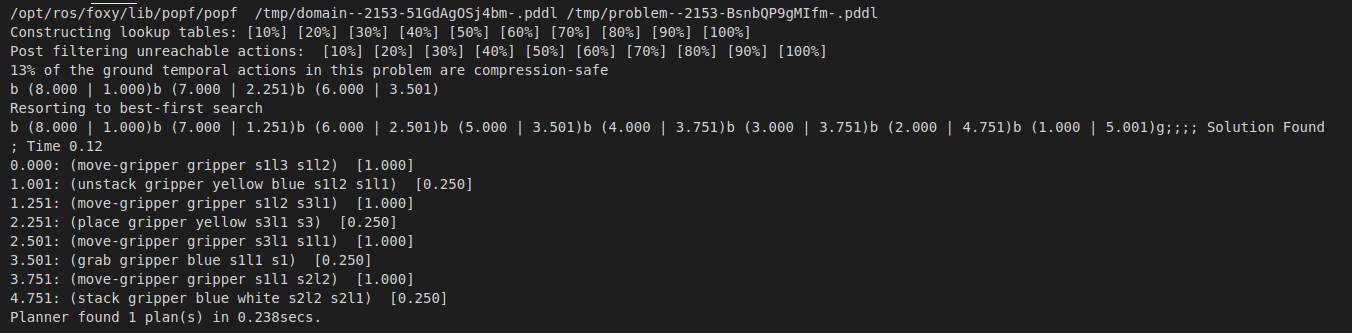
\includegraphics[width=\textwidth]{plugin_plan}
    \caption{Konsolenausgabe nach Ausführung des Planers über das PDDL-Plugin}
    \label{fig:pluginplan}
\end{figure}

\begin{figure}[ht!]
    \centering
    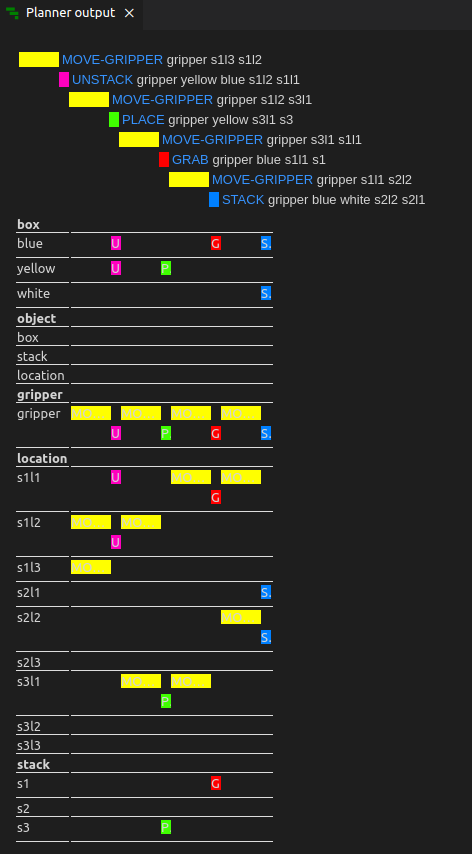
\includegraphics[width=\textwidth]{plugin_vis}
    \caption{Visualisierung eines Plans mit dem PDDL-Plugin}
    \label{fig:pluginvis}
\end{figure}
\subsubsection{Partial Order Planning}{\label{section:pop}}
\ac{POP} ist eine Form des Planens, in dem die Aktionen eines Plans nur soweit geordnet sind, wie es notwendig ist \cite{dyer_2003}.
Dies steht im Gegensatz zu Total-Order Planern wie \ac{STRIPS}.\\
Es wird nach dem Principle Of Least Commitment verfahren.
Das bedeutet, dass Entscheidungen soweit wie möglich aufgeschoben und erst getroffen werden, wenn es absolut nötig ist.
Dies umfasst nicht nur die Reihenfolge von Aktionen, sondern auch die Bindung von Variablen.\\
Ein Partial-Order Plan kann als 4-Tupel \cite{grastien} beschrieben werden.
\begin{itemize}
    \item eine Menge von Aktionen
    \item eine Menge von Einschränkungen der Reihenfolge
    \item eine Menge von kausalen Zusammenhängen
    \item eine Menge offener Vorbedingungen (Vorbedingungen einer Aktion, die nicht durch eine andere Aktion erfüllt werden)
\end{itemize}
Die Menge der Aktionen enthält Instanzen von Aktionen der Domäne.
Eine Aktion der Domäne kann daher mehrfach vorkommen.
Einschränkungen der Reihenfolge $A < B$ bilden ab, dass Aktion $A$ vor Aktion $B$ ausgeführt werden muss.
Zyklische Einschränkungen sind nicht erlaubt.
Ein kausaler Zusammenhang $A \xrightarrow{\alpha} B$ beschreibt, das die Aktion $A$ die Vorbedingung $\alpha$ der Aktion $B$ erfüllt.\\
Die Suche erfolgt im Plan Space.
Jeder Knoten im Graph entspricht einem Teilplan und jede Kante einer Änderung des einen zum anderen Plan.
Dies kann durch das Hinzufügen eines weiteren Schrittes oder einer Einschränkung sowie der Bindung einer Variable geschehen.
Die Wurzel des Graphen besteht aus einem Plan mit zwei Schritten, die den Startzustand und das Ziel darstellen.
Der Startzustand wird durch eine Aktion repräsentiert, die keine Vorbedingungen und alle Fakten als Effekt hat.
Das Ziel erhält alle Zielfakten als Vorbedingung und hat keinen Effekt.
Zusätzlich enthält der Plan die Einschränkung, dass die Aktion für den Start vor der für das Ziel ausgeführt werden muss ($Start < Ziel$).\\
Ein Plan ist eine Lösung, wenn \cite{grastien}:
\begin{itemize}
    \item keine Aktion des Plans eine offene Vorbedingung hat
    \item und wenn keine Threats existieren
\end{itemize}
Ist der aktuelle Plan keine Lösung werden folgende Schritte vorgenommen~\cite{grastien}:
\begin{itemize}
    \item eine offene Vorbedingung $p$ einer Aktion $B$ wählen
    \item eine existierende Aktion $A$, die die Vorbedingung $p$ erfüllt wählen oder eine neue Aktion $A$ erzeugen
    \item den kausalen Zusammenhang $A \xrightarrow{p} B$ und die Reihenfolge $A < B$ hinzufügen
    \item wenn $A$ eine neue Aktion ist, die Reihenfolge $Start < A$ hinzufügen
    \item Probleme zwischen dem neuen kausalen Zusammenhang und den existierenden Aktionen lösen sowie zwischen den existierenden kausalen Zusammenhang und $A$, wenn $A$ eine neue Aktion ist.
    \item entsteht durch das Hinzufügen der Reihenfolgen ein Zyklus kann der Plan keine Lösung mehr werden
\end{itemize}
Ein Problem ist eine Beziehung zwischen einer Aktion $C$ und einem kausalen Zusammenhang  $A \xrightarrow{p} B$, bei der die Aktion $C$ einen Effekt $\neg p$ hat.
Sollte $C$ nach $A$ aber vor $B$ ausgeführt werden, ist die Vorbedingung $p$ für $B$ nicht mehr gegeben.
Probleme können durch \emph{Promotion} oder \emph{Demotion} gelöst werden~\cite{dyer_2003}.
Bei \emph{Promotion} wird der problematische Schritt $C$ nach dem kausalen Zusammenhang ausgeführt: die Reihenfolge $B < C$ wird hinzugefügt.
Bei \emph{Demotion} wird der problematische Schritt $C$ vor dem kausalen Zusammenhang ausgeführt: die Reihenfolge $C < A$ wird hinzugefügt.

\subsubsection{Forward Chaining Partial Order Planning}
Die Prinzipien des \ac{POP} sollen nun mit Vorwärtsverkettung kombiniert werden.
%Speziell soll das temporale Planen mit Metriken optimiert werden.
Für Vorwärtsverkettung mit einem Total-Order Plan können Zustände als Tupel $(F,V,Q,P,C)$ beschrieben werden~\citep{popf}:
\begin{itemize}
    \item F ist eine Menge von Fakten die im Zustand gelten
    \item V enthält die Werte numerischer Variablen
    \item Q ist eine List von Aktionen die begonnen haben aber noch nicht beendet sind
    \item P ist der Plan um den Zustand zu erreichen
    \item C ist eine Liste aller zeitlichen Einschränkungen der Schritte in $P$
\end{itemize}
Um eine Aktion zum Plan hinzuzufügen müssen deren Start- und Endpunkte hinzugefügt werden.
Dies muss nicht in aufeinander folgenden Schritten geschehen.
Wird eine Aktion hinzugefügt werden $F$ und $V$ entsprechend der Effekte angepasst.
Die Voraussetzung um eine Aktion hinzufügen zu können ist, dass $Q$ keine Aktion enthält, zu der die Effekte der neuen Aktion einen Konflikt darstellen würden.\\
Vorwärtsverkettung im Zustandsraum hat, durch den Total-Order Plan, den Vorteil, dass nicht explizit nach Problemen gesucht werden muss.
Neue Aktionen werden immer am Ende hinzugefügt, wodurch sie kein Problem für die Vorbedingungen und Effekt früherer Aktionen darstellen können.
Gleichzeitig kann keine folgende Aktion ein Problem für diese darstellen.
Dieser Vorteil kommt mit dem Nachteil der frühen Bindung und einer festgelegten Reihenfolge zwischen Aktion, zwischen denen kein Zusammenhang besteht.\\
Es soll ein Kompromiss zwischen den Vorteilen von Total- und Partial-Order Planung gefunden werden.
Dem Tupel werden weitere Elemente hinzugefügt:
\begin{itemize}
    \item $F^+(F^-)$, wobei $F^+(p)(F^-(p))$ den Index eines Schrittes $a$ angeben, indem der Fakt $p$ als letztes hinzugefügt (oder gelöscht) wurde
    \item $FP$, wobei $FP(p)$ eine Menge von Paaren $\langle i,d \rangle \in (\mathbb{N}_0 \times \{0,\epsilon\})$:\\
    \begin{itemize}
        \item $\langle i,0 \rangle \in FP(p)$ beschreibt, dass Schritt $i$ am Ende eines offenen Intervalls liegt, in dem $p$ wahr sein muss.\\
        In \ac{PDDL} gibt es diese für Aktionen mit der \emph{over all} Bedingung $p$, wobei $i$ der Endpunkt dieser Aktion ist.
        \item $\langle i,\epsilon \rangle \in FP(p)$ beschreibt, dass Schritt $i$ der Start eines Intervalls ist, indem $p$ wahr sein muss.\\
        Dies entspricht \emph{at start} oder \emph{at end} Bedingungen in \ac{PDDL} die relevant für den Schritt $i$ sind.
    \end{itemize}
\end{itemize}
Diese Methodik wird in dem am King’s College London entwickelten Planer \ac{POPF} implementiert.
%\subsubsection{Partial Order Planning Forward}
%\ac{POPF} ist ein am King’s College London entwickelter Planer, der die in Abschnitt~\ref{section:pop} genannten Methoden implementiert~\citep{popf}.
%Es wird ein temporaler \ac{RPG} genutzt.
%Ein \ac{RPG} ist ein Planungsgraph, in dem negative Effekte von Aktionen ignoriert werden.
%Der Graph besteht aus Aktions- und Faktenschichten, die sich abwechseln.
%Die Wurzel des Graphen ist eine Faktenschicht, die den aktuellen Zustand abbildet.

\subsubsection{Behavior Tree}
\acp{BT} sind ein modulares System, das in der Videospieleindustrie entwickelt wurde~\cite{bt_book}.
Sie ermöglichen aus simplen Aktionen komplexe Verhaltensmuster zu modelieren ohne das Aktionen Kenntnis über andere Aktionen haben müssen~\cite{bt_robotics}.
Ein \ac{BT} ist ein gerichteter azyklischer Graph $G(V,E)$ mit $|V|$ Knoten und $|E|$ Kanten.
Ein Eltern Knoten von einem Paar verbundener Knoten ist der, von dem die Kante ausgeht.
Der Knoten mit der eingehenden Kante ist ein Kind Knoten.
Knoten ohne Kinder heißen Blätter.
Ein Knoten ohne Eltern heißt Wurzel.
In einem \ac{BT} gibt es genau eine Wurzel mit genau einem Kind~\cite{bt_1}.\\
Die Ausführung eines \ac{BT} beginnt bei der Wurzel, die in einem bestimmten Intervall ein Signal erzeugt, dass die Ausführung eines Knoten erlaubt (''tick'').
Dieses Signal wird an das Kind der Wurzel gesendet.
Ein Knoten wird ausgeführt, wenn es dieses Signal erhält und auch nur dann.~\cite{bt_book}
Wird ein Knoten ausgeführt, gibt er einen Status zurück.
Der Status ist einer von drei möglichen~\cite{bt_uav}:
\begin{itemize}
    \item Running: die Ausführung läuft noch
    \item Success: die Ausführung war erfolgreich
    \item Failure: die Ausführung ist fehlgeschlagen
\end{itemize}
Blätter sind Ausführungsknoten und haben einen der folgenden Typen:
\begin{itemize}
    \item Aktion
    \item Bedingung
\end{itemize}
Knoten mit Kindern, mit Ausnahme der Wurzel, sind Kontrollfluss Knoten und haben einen der folgenden Typen~\cite{bt_1}:
\begin{itemize}
    \item Selektor
    \item Sequenz
    \item Parallel
    \item Dekorator
\end{itemize}
Ein Selektor Knoten führt seine Kinder der Reihe nach aus bis das erste einen Status \emph{Running} oder \emph{Success} zurückgibt.
Nachfolgende Kinder werden dann nicht mehr ausgeführt und der Selektor gibt den entsprechenden Status zurück.
Wurden alle Kinder ausgeführt und keins hat einen Status \emph{Running} oder \emph{Success} zurückgegeben, gibt der Selektor den Status \emph{Failure} zurück.\\
Ein Sequenz Knoten führt seine Kinder der Reihe nach aus, bis das erste einen Status \emph{Running} oder \emph{Failure} zurückgibt.
Nachfolgende Kinder werden dann nicht mehr ausgeführt und die Sequenz gibt den entsprechenden Status zurück.
Wurden alle Kinder ausgeführt und keins hat einen Status \emph{Running} oder \emph{Failure} zurückgegeben, gibt die Sequenz den Status \emph{Success} zurück.\\
Ein Parallel Knoten führt alle Kinder aus, ohne auf den Status des vorherigen zu warten.
Überschreitet die Anzahl der Kinder die \emph{Success} zurückgeben einen benutzerdefinierten Wert $S$ gibt der Knoten \emph{Success} zurück.
Haben $N-M+1$ Kinder \emph{Failure} zurückgegeben, wobei $N$ die Anzahl der Kinder ist, wird \emph{Failure} zurückgeben, da der Wert $S$ nicht mehr erreicht werden kann~\cite{bt_book}.
Alternativ kann ein zweiter benutzerdefinierter Wert $F$ eingeführt werden.
Überschreitet die Anzahl der Kinder die \emph{Failure} zurückgeben diesen Wert $F$ wird direkt \emph{Failure} zurückgegeben~\cite{bt_1}.
$S$ und $F$ müssen $\leq M$ sein.
Wird keiner dieser beiden Werte überschritten, wird \emph{Running} zurückgegeben.\\
Ein Dekorator Knoten hat genau ein Kind.
Er kann durch eine Bedingung entscheiden ob das Kind ausgeführt wird und kann einen modifizierten Status zurück geben.
Beispiele für Dekoratoren sind:
\begin{itemize}
    \item Invertierung/Negation: der \emph{Success} und \emph{Failure} Status des Kinds wird invertiert
    \item Zeitbeschränkung: gibt das Kind den Status \emph{Running} für länger als eine benutzerdefinierter Zeitspanne $T$ zurück, wird \emph{Failure} zurückgegeben und das Kind nicht mehr ausgeführt
\end{itemize}\cite{bt_book}
- Visualisierungs bsp.\\
\subsubsection{PlanSys2}
- Theoretischen/Grundlagen-Teil von Impl. hierher verschieben\\
- config für andere Planer\\
\ac{PlanSys2} ist ein modulares Planungsframework für \ac{ROS2}.
Ursprünglich als Nachfolger für ROSPlan~\cite{rosplan} geplant, bietet es viel umfangreichere Funktionen~\cite{plansys}.
Hierfür werden unter anderem neue Funktionen von \ac{ROS2} wie LifeCycle Knoten oder Multicast Kommunikation genutzt.\\
Eins der Designprinzipien bei der Entwicklung von \ac{PlanSys2} ist Modularität und Erweiterbarkeit.
Alle Komponenten haben klar definierte Schnittstellen, wodurch sie einfach erweitert oder ausgetauscht werden können.\\
Die Hauptkomponente ist der \emph{Planner} Knoten, der den tatsächlichen Planer aufruft.
Verschiedene Planer können über Plugins aufgerufen werden, die beschreiben, wie der Planer aufzurufen ist und wie der generierte Plan zu verstehen ist.
Standardmäßig sind \ac{POPF} sowie TFD (Temporal Fast Downward)~\cite{tfd} verfügbar und konfiguriert.\\
Der \emph{Domain Expert} Knoten liest die Domäne im \ac{PDDL} Format ein.
Er kann mehrere verschiedene Domänen zu einer kombinieren.
Dies ermöglicht es mehrere modulare Packages zu nutzen, die jeweils nur den für sie relevanten Teil einer Domäne beinhalten sowie deren Aktionen  implementieren.
Der Knoten dient zur Validierung (z.B. ob ein Prädikat, dass hinzugefügt werden soll mit den gegeben Objekten gültig ist) und dem Planer die Domäne zur Verfügung zu stellen.\\
Der \emph{Problem Expert} Knoten enthält alle Informationen zum gegebenen Problem: Objekte, Prädikate, Funktionen und Ziele.
Diese werden immer über den \emph{Domain Expert} validiert.
Wenn ein Plan angefordert wird, werden die gespeicherten Informationen zu einem Problem im \ac{PDDL} Format konvertiert und dem \emph{Planner} Knoten zur Verfügung gestellt.\\
Der \emph{Executor} Knoten ist dafür zuständig einen generierten Plan auszuführen.
Der Plan wird in einen \ac{BT} konvertiert, der diesen ausführt.